\documentclass[12pt,a4]{article}
\usepackage[left=1.8cm,right=1.8cm,top=32mm,columnsep=20pt]{geometry}

\usepackage[utf8]{inputenc} %Formato de codificación
\usepackage[spanish, es-tabla, es-nodecimaldot]{babel}
\usepackage{amsmath} %paquete para escribir ecuaciones matemáticas
\usepackage{float} %Para posicionar figuras
\usepackage{graphicx} %Para poder poner figuras
\usepackage{hyperref} %Permite usar hipervínculos
\usepackage{multicol} %Para hacer doble columna
\usepackage[sorting=none]{biblatex} %Imports biblatex package. To cite use \cite{reference_label}
\usepackage{csquotes}

\title{Informe de Física: Encontrando el coeficiente de fricción dinámica}
\author{Francisco Carruthers, Facundo Firpo y Joel Jablonski\\ [2mm] %\\ para nueva línea
\small UDESA}
\date{2do Semestre 2024}


\begin{document}

\maketitle

\begin{abstract}
    Utilizando un carrito, una soga y una polea, se busca encontrar el coeficiente de fricción dinámica entre el carrito y la superficie. Para ello, se mide la aceleración del carrito con distintas masas y se calcula el coeficiente de fricción dinámica. También, utilizamos varias superficies para ver cómo afecta el coeficiente de fricción.
\end{abstract}

\section{Introducción}

Medimos los datos usando un Arduino

\newpage
\section{Calibración}

Utilizamos un sistema de referencia para calibrar el sistema.

\begin{figure}[H]
    \centering
    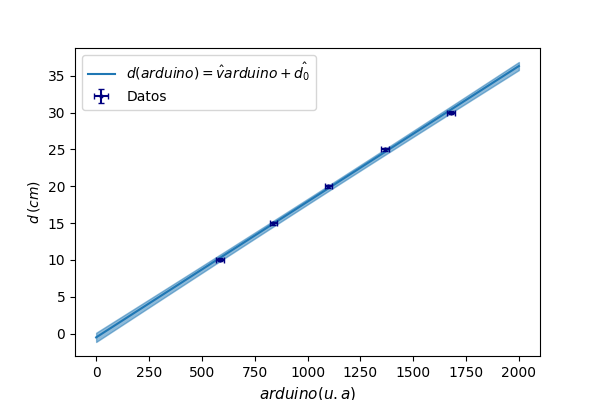
\includegraphics[width=0.9\linewidth]{Calibracion.png}
    \caption{Calibración del sistema}
    \label{fig:calibracion}
\end{figure}

Pendiente: 0.0184 ± 0.0005 \\

Ordenada al origen: -0.508 ± 0.532 \\

Distancia para 600: 10.54 ± 0.44 cm \\

\section{Resultados}

\end{document}